The results from this study indicate that there is a significant effect on the
utility of elastic deformation as a data augmentation technique, for the
segmentation of 2-d echocardiography frames. What is not evident in the data as
presented is the utility of a C-GAN in the data augmentation step. However there
are some noteworthy observations of the study, which present new information.\newline

The model architecture was intentionally not optimised specifically for the
problem domain, beyond a base-level accuracy. The logic behind this being that
the effect of data augmentation on a very-well architected network, which would
already achieve a very high baseline accuracy, may not be particularly
significant. However in the general case, potentially when segmenting noisier
images or a higher resolution modality with more classes, where baseline
accuracy is lower, the utility would be more evident. Therefore the main
hypothesis of this study, whether generated images were superior to simply
elastically deformed images for data augmentation is disproven.
Further work in the area would be needed to establish this as a rule.
\newline

The end results of the study do not align with what intuitively the endpoints
should have been however. See Figure \ref{fig:conditional} below, where it is clear that the
generated image has a closer approximation to a real echocardiography frame (as
the ultrasound window has not also been deformed). \newline

\begin{figure}[H]
    \centering
    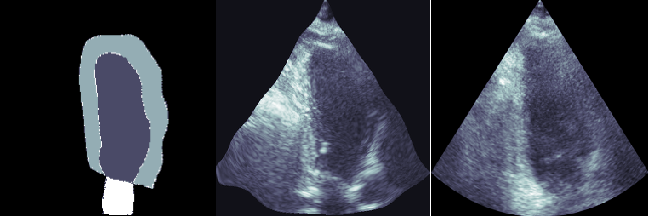
\includegraphics[width=1.0\textwidth]{figures/conditional.png}
    \caption{Left - Deformed conditional input to GAN, Middle - Real deformed image, Right - Fake generated image from deformed condition}
    \label{fig:conditional}
\end{figure}

Other notable observations about the types of images is the generated image is
(expectedly) substantially noisier than the real image. This could potentially
be mitigated by contrast and other augmentations, but would require further
investigation. One of the key advantages of the C-GAN augmentation is
maintaining the ultrasound window shape (in the Middle image, the ultrasound
window has very clearly been deformed as part of the elastic deformation
process). However the experimental results of this work would suggest that this
did not have a substantial effect - a possible explanation for this is the
encoder phase of the segmentation neural network would not have much "attention"
on this part of the image. This would particularly be the case on models trained
with the weighted cross entropy loss function, which the final baseline model
had been. Another final observation of the generated image, is its observed
matching of the segmentation mask boundaries to the photorealistic
representation. \newline

Mathematically there are two ways to consider this; is the generator learning
the transfer function mapping the set of conditions (segmentation masks) to the
set of photorealistic representations, or is the generator learning the
conditional probability distribution of the likely photorealistic image given an
input condition? \newline

We model the first interpretation in Equation 4. The first interpretation would
be the superior and far more general interpretation of how the generator is
learning within the C-GAN framework. \newline 

\begin{equation}
    G: C \rightarrow P
\end{equation} \newline

Generator as a transfer function, where $G$ is the generator trained by the
C-GAN, $C \in \{0,1\}^{256\times256\times4}$ (the conditional input) and $P \in
\mathbb{R}^{256\times256}$ (the photorealistic output) \newline


Or there is an alternate interpretation which is the generator is learning the
conditional probability distribution as shown in Equation 5. This
interpretation is less general and rigorous, and is the prevalent interpretation
in literature. \newline

\begin{equation}
    G_{P|C}(c) = p
\end{equation} \newline

Generator as a conditional probability distribution, where $G$ is the generator
trained by the C-GAN, $C \in \{0,1\}^{256\times256\times4}$ (the conditional
input) and $P \in \mathbb{R}^{256\times256}$ (the photorealistic output) and $p
\in P, c \in C$ \newline

It would be far out of the scope of this body of work to propose that the first
intepretation is applicable in this scenario. However given the generator
trained in our work appears to be able to generate non-physiological
photorealistic echocardiography frames from deformed conditions, it is not an
unreasonable speculation. This could potentially be enforced by using a loss
function which is being optimized for some physical metric, such as the
Haussdorf distance. \newline

To validate the proposal of mathematically describing the generator as a loss
function, analysing the quantitative effect of linearly scaling the input
condition would give useful results. \newline 

There are some outlying limitations of this study, namely an analysis of whether
the data augmentation methods improved the measurement of the end clinical
indices. This would be good further direction for this study, but was not
included in the scope of this work. This is in part as it is still speculative
whether a segmentation approach is superior for the measurement of clinical
indices for echocardiography. 3D convolution approach have seen increasing usage
in literature, and are converging on similar accuracy rates as segmentation
approaches. By focussing on the segmentation accuracy, this study remains
generalizable to semantic segmentation broadly - rather than just the
measurement of echocardiography clinical indices. \newline

Another limitation of this study is the same as our comment on the work Abdi et
al. which is not providing a metric of the accuracy of the generator network.
Overlap scores such as IoU would give an interesting analysis of the generator,
and potentially provide further evidence for the prior speculation of the
transfer function vs conditional probability distribution argument. \newline

A further limitation for this study is the loss function potentially was
not aligned with the endpoint of the study. A training graph excerpted from
TensorBoard is provided below in Figure \ref{fig:tboard}

\begin{figure}[H]
    \centering
    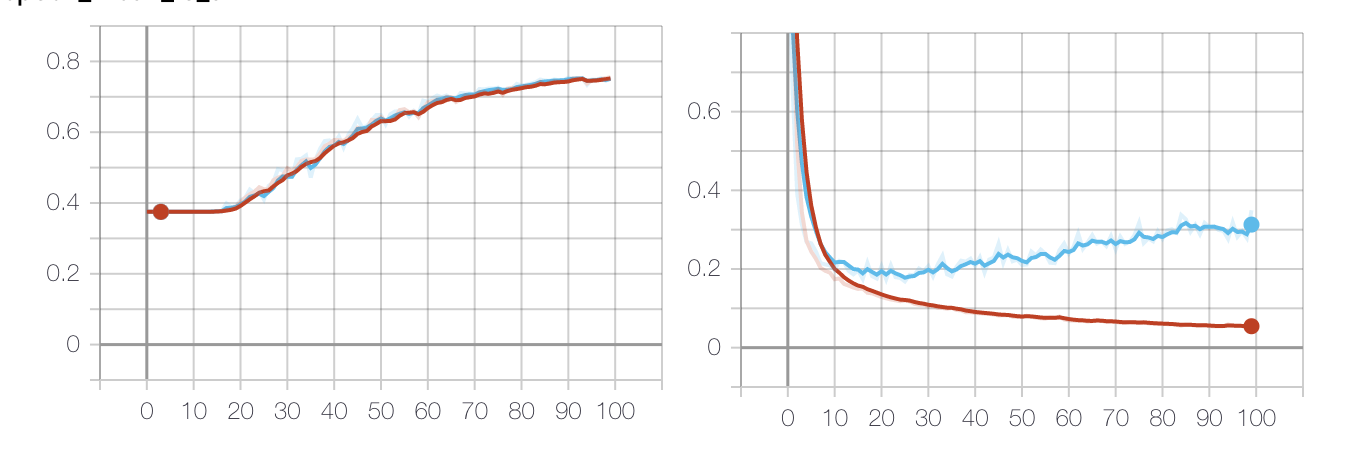
\includegraphics[width=1.0\textwidth]{figures/train.png}
    \caption{Left - Mean IoU, Right - Weighted Categorical Cross Entropy. In both graphs, red for training data, blue for testing data.}
    \label{fig:tboard}
\end{figure}

As can be seen, although the loss function (Weighted Categorical Cross Entropy,
WCCE) would suggest overfitting, one of the accuracy metrics tracked by
TensorBoard - Mean IoU - is still improving. Given mIoU is more closely aligned
with this studies endpoint of improved segmentation accuracy, this suggests a
review of the convergence criteria is needed. During the development of the
baseline model, we did experiment with the use of mIoU as a loss function - but
found little success and the model seemed to learn little in early epochs.
Potentially a hybrid method would see success - train the model on WCCE until a
certain level of accuracy, before using mIoU for further tuning - but was not
investigated in this work and would be good further direction for the study.
\newline

The final limitation we identified with this study is the results potentially
showing the utility of data augmentation broadly, in simply providing the model
with more samples to learn on during training. This effect would be seen
regardless of the augmentation method used. Future work of interest would be
comparing the use of C-GANs and more conventional data augmentation techniques -
such as rotation, flipping and contrast enhancement - however were not applied
in this study out of interest of maintaining a single independent variable.
\newline

In summary, this body of work gives evidence of elastic deformation being a valuable
data augmentation technique for the segmentation of echocardiography frames.
This partially proves our initial hypothesis. This body of work has not given
evidence to suggest the use of a C-GAN is a superior data augmentation
technique, and further work would be needed to prove or disprove this. \newline